\documentclass{beamer}
\usepackage{graphicx}
\usepackage{paralist}
\usepackage{outlines}

\title{Table of Contents - Week 10}
\author{Mendocino College - Digital Image Manipulation with Photoshop}
\titlegraphic{\vspace{-10mm}
\includegraphics[width = .9\textwidth]{images/photoshop.jpg}} 
\date{\vspace{-5em}} 


\mode <presentation>
\usetheme{Warsaw}
\usecolortheme{default}

\setbeamerfont{footline}{size=\fontsize{5}{8}\selectfont}

\definecolor{darkred}{rgb}{20,0,0}
\definecolor{darkgreen}{RGB}{40,110,20}
\definecolor{darkpurple}{RGB}{30,0,30}
\definecolor{chardonnay}{RGB}{255, 255, 204}

\setbeamercolor*{palette primary}{fg=white, bg=darkgreen}


\begin{document}
	{
		\setbeamertemplate{footline}{} 
		\setbeamertemplate{headline}{} 
		\begin{frame}
			\vspace{-35pt}
			\maketitle
		\end{frame}
	}

		\section{Announcements}
			\subsection{Opening Lab Earlier}		
			\begin{frame}
				\frametitle{Lab Will be Open Earlier}
				\begin{columns}
					\column{.6\textwidth}
					\vspace{-25pt}
					\begin{outline}
						\1 We only have 2.5 hours of classtime per week.
						\1 I will be opening the lab earlier before class to help students complete their assignments.
						\1 7:50am: Monday Tuesday Thursday.
						\1 If requested, we can open as early as 7:30am
					\end{outline}
					\column{.45\textwidth}
					
\includegraphics[width=0.9\textwidth]{images/F0136159-Businessman_working_at_computer_at_desk.jpg}
				\end{columns}
			\end{frame}
			
			\subsection{College Day}		
			\begin{frame}
				\frametitle{College Day at the Coast Center}
				\begin{outline}
					\1 Learn about Opportunities at Mendocino College
					\1 Transfer Talk
					\1 Health Talk
					\1 Prizes
				\end{outline}
				
\includegraphics[width=0.9\textwidth]{images/college day.png}
			\end{frame}

	\section{Lecture Topics}
			\subsection{Lecture Topics}		
	\begin{frame}
		\frametitle{Lecture Topics for Week 10}
				\begin{outline}
					\1 Colour Sampling Tools
					\1 Replacing Colours
					\1 Colour Correction
					\1 Visual Design Principles
				\end{outline}
		\end{frame}

			\subsection{Colour Sampling Tools}		
				\begin{frame}
					\frametitle{Colour Sampling Tools}
					\begin{outline}
						\1 Eyedropper Tool
						\1 Color Sampler Tool
						\1 Color Picker
					\end{outline}
					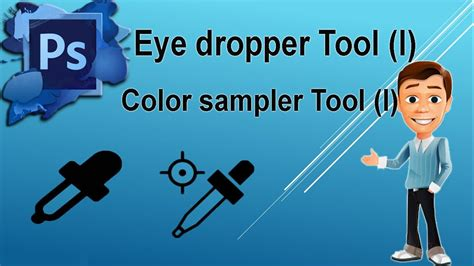
\includegraphics[width=1.0\textwidth]{images/color sampling tools.jpg}
				\end{frame}
			
		\subsection{Colour Correction}		
			\begin{frame}
				\frametitle{Colour Correction}
				\begin{outline}
					\1 Curves adjustment layer
					\1 Levels adjustment layer
					\1 Auto Correction Options
					\1 "4-Point" technique
					\1 Adobe Bridge and Camera Raw
				\end{outline}
			
\includegraphics[width=0.8\textwidth]{images/color correction.jpg}
			\end{frame}
			

			\subsection{Replacing Colours}		
				\begin{frame}
					\frametitle{Changing Colours}
					\begin{outline}
						\1 Making Selections and using Masks
						\1 Using Solid Colors and Blending Modes
						\1 Curves \& Levels adjustment layers
						\1 Hue / Saturation adjustment layers
					\end{outline}
				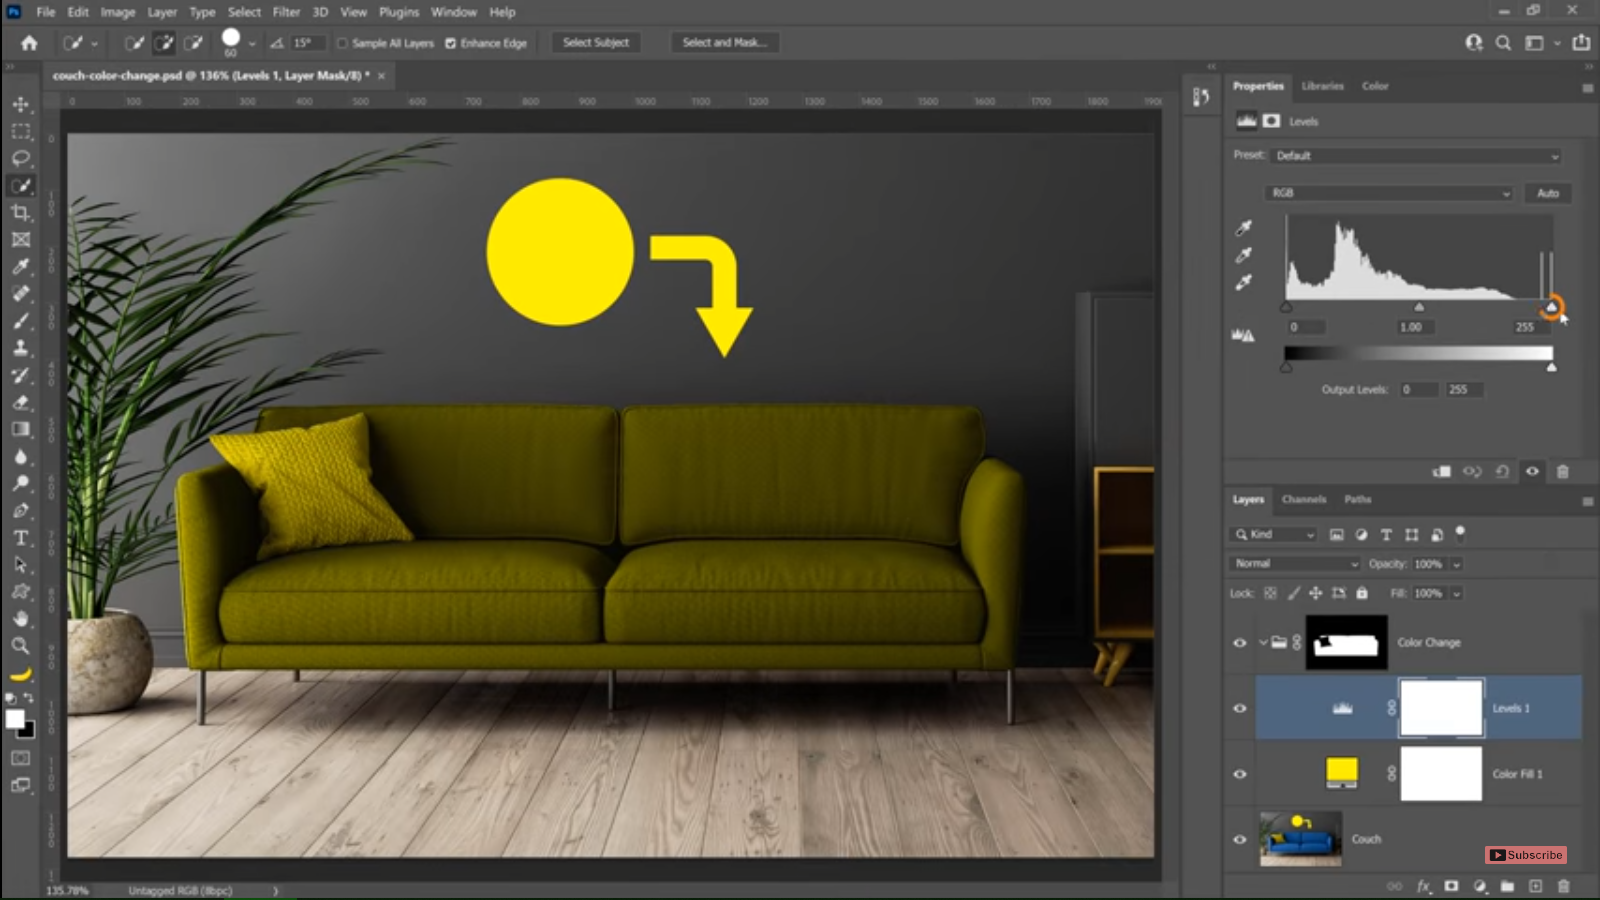
\includegraphics[width=0.9\textwidth]{images/color change.png}
				\end{frame}


			\subsection{Visual Design Principles}		
				\begin{frame}
					\frametitle{Visual Design Principles}
					\begin{columns}
						\column{.6\textwidth}
						\vspace{-25pt}
						\begin{outline}
							\1 The elements and principles of visual design and composition: 
							\2 Balance, Leading Lines, Texture, 
							\2 Color/Contrast, Negative Space, 
							\2 Emphasis, Point of View,
							\2 Strong Focal Point, Emphasis,
							\2 Pattern, Repetition, 
							\2 Alignment, etc.
						\end{outline}
						\column{.45\textwidth}
						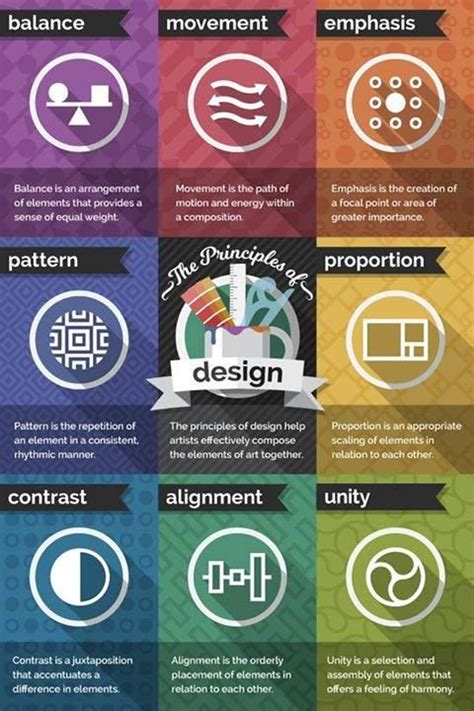
\includegraphics[width=1.0\textwidth]{images/principles of design.jpeg}
					\end{columns}
					
				\end{frame}
			
		\section{Assignments}
			\subsection{Weekly Exercises}		
			\begin{frame}
				\frametitle{Exercises for Week 10}
				\begin{outline}
					\1 Correcting Colors with Levels and Curves
					\1 Auto Color Correction Options
					\1 Changing the color of a selected object
					\1 Applying Design Principles
				\end{outline}
				\includegraphics[width=0.5\textwidth]{images/auto color correction - levels.png}
			\end{frame}
		
		\subsection{Assignment}		
			\begin{frame}
				\frametitle{Colour Correction Assignment}
				\begin{outline}
					\1 We will be using Adobe Bridge and Camera Raw
					\1 Manually Correct a Photo using Camera Raw
					\1 Explain all the changes you made
				\end{outline}
			\includegraphics[width=0.8\textwidth]{images/BARNARD_CS7011B_Class2.png}
			\end{frame}
	
		\section{Discussion}
			\subsection{Readings \& Videos}		
				\begin{frame}
					\frametitle{Videos \& Articles}
					\begin{outline}
						\1 YouTube Video:  How to Change Color in Photoshop
							\2 By:  Photoshop Training Channel
							\2 Duration:  17 minutes and 40 seconds
						\1 YouTube Video:  The Complete Color Correction Process in Photoshop
							\2 By:  PiXimperfect
							\2 Duration:  18 minutes and 36 seconds
						\1 Article:  8 Essential Visual Principles Explained
							\2 By:  Andrew Wilshere
							\2 Pages:  29
					\end{outline}
					
				\end{frame}

			\subsection{Research Topics}		
				\begin{frame}
					\frametitle{Research Topics}
					\begin{columns}
						\column{.5\textwidth}
						\begin{outline}
							\1 Eyedropper Tool
							\1 Color Sampler Tool
							\1 Tone
							\1 Contrast
							\1 Hue
							\1 Saturation
							\1 Levels adjustment layer
							\1 Curves adjustment layer
						\end{outline}
						\column{.5\textwidth}
					\begin{outline}
						\1 Balance (design principle)
						\1 Movement (design principle)
						\1 Emphasis (design principle)
						\1 Pattern (design principle)
						\1 Proportion (design principle)
						\1 Contrast (design principle)
						\1 Alignment (design principle)
						\1 Unity (design principle)
					\end{outline}
					\end{columns}
				\end{frame}
	
	\section{}	
		\subsection{End Card}
		\begin{frame}
			\frametitle{End Card}	
			\begin{columns}
				\column{.6\textwidth}
				\vspace{-25pt}
				\begin{itemize}
					\item Joshua Paul Barnard
					\item Computer Science Instructor
					\item Mendocino College
				\end{itemize}
			\space
				\begin{itemize}
					\item Presentation was made in \LaTeX
					\item For the Fall 2022 semester.  
				\end{itemize}
				\begin{itemize}
					\item jbarnard@mendocino.edu
					\item github.com/JoshuaPaulBarnard
				\end{itemize}
				\column{.45\textwidth}
				
\includegraphics[width=.85\textwidth]{images/shone farm wine pouring - vert.png}
			\end{columns}
		\end{frame}
	
\end{document}